% fig_mc_dependability.tex
% TR-37: Dependability and mean clearance time by TR-29 region and fault type
% Two grouped bar charts side by side using pgfplots
%
% Left: P_dep by region (A=0.9709, B=1.000, C=1.000, D=1.000)
% Right: P_dep by fault type (3PH=0.9453, SLG=1.000, LL=1.000, LLG=1.000)

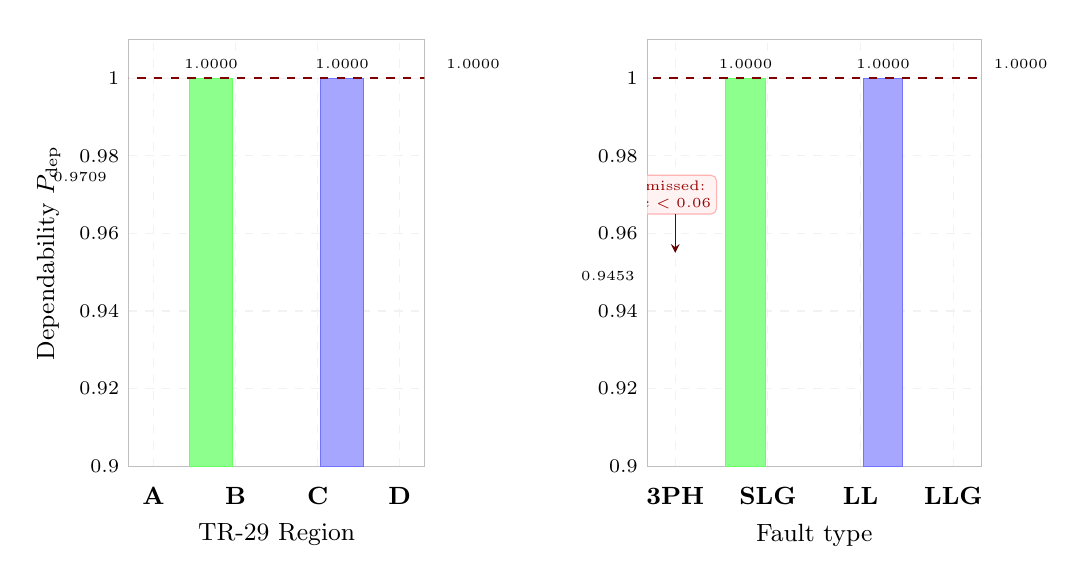
\begin{tikzpicture}
\begin{axis}[
  name         = regax,
  width        = 0.44\textwidth,
  height       = 7.0cm,
  ybar,
  bar width    = 0.55cm,
  xlabel       = {TR-29 Region},
  ylabel       = {Dependability $P_\mathrm{dep}$},
  xlabel style = {font=\small},
  ylabel style = {font=\small},
  ymin=0.90, ymax=1.010,
  ytick        = {0.90,0.92,0.94,0.96,0.98,1.00},
  yticklabel style={font=\scriptsize},
  xtick        = {1,2,3,4},
  xticklabels  = {A, B, C, D},
  xticklabel style={font=\small\bfseries},
  tick style   = {draw=none},
  axis line style={gray!50},
  grid         = major,
  grid style   = {gray!10, dashed},
  nodes near coords,
  nodes near coords style={font=\tiny, anchor=south},
  every node near coord/.append style={
    /pgf/number format/.cd, fixed, fixed zerofill, precision=4
  },
]

%% Region bars
\addplot[fill=gray!40,  draw=gray!60]    coordinates {(1, 0.9709)};
\addplot[fill=green!45, draw=green!60]   coordinates {(2, 1.0000)};
\addplot[fill=blue!35,  draw=blue!55]    coordinates {(3, 1.0000)};
\addplot[fill=teal!40,  draw=teal!60]    coordinates {(4, 1.0000)};

%% Reference line at 1.0
\draw[red!50!black, dashed, thick] (axis cs:0.4,1.0) -- (axis cs:4.6,1.0);

\end{axis}

\begin{axis}[
  name         = ftax,
  at           = (regax.right of south east), anchor=left of south west,
  xshift       = 8mm,
  width        = 0.48\textwidth,
  height       = 7.0cm,
  ybar,
  bar width    = 0.50cm,
  xlabel       = {Fault type},
  ymin=0.90, ymax=1.010,
  ytick        = {0.90,0.92,0.94,0.96,0.98,1.00},
  yticklabel style={font=\scriptsize},
  xtick        = {1,2,3,4},
  xticklabels  = {3PH, SLG, LL, LLG},
  xticklabel style={font=\small\bfseries},
  xlabel style = {font=\small},
  tick style   = {draw=none},
  axis line style={gray!50},
  grid         = major,
  grid style   = {gray!10, dashed},
  nodes near coords,
  nodes near coords style={font=\tiny, anchor=south},
  every node near coord/.append style={
    /pgf/number format/.cd, fixed, fixed zerofill, precision=4
  },
]

\addplot[fill=red!35,    draw=red!55]    coordinates {(1, 0.9453)};
\addplot[fill=green!45,  draw=green!60]  coordinates {(2, 1.0000)};
\addplot[fill=blue!35,   draw=blue!55]   coordinates {(3, 1.0000)};
\addplot[fill=purple!35, draw=purple!55] coordinates {(4, 1.0000)};

\draw[red!50!black, dashed, thick] (axis cs:0.4,1.0) -- (axis cs:4.6,1.0);

%% Annotation: 3PH misses at low k
\node[red!60!black, font=\tiny, align=center, draw=red!30, fill=red!5,
      rounded corners=2pt, inner sep=2pt]
  at (axis cs:1.0, 0.970)
  {missed:\\$k<0.06$};
\draw[->, >=stealth, red!40!black, thin]
  (axis cs:1.0, 0.965) -- (axis cs:1.0, 0.955);

\end{axis}
\end{tikzpicture}
